

\tikzset{every picture/.style={line width=0.75pt}} %set default line width to 0.75pt        

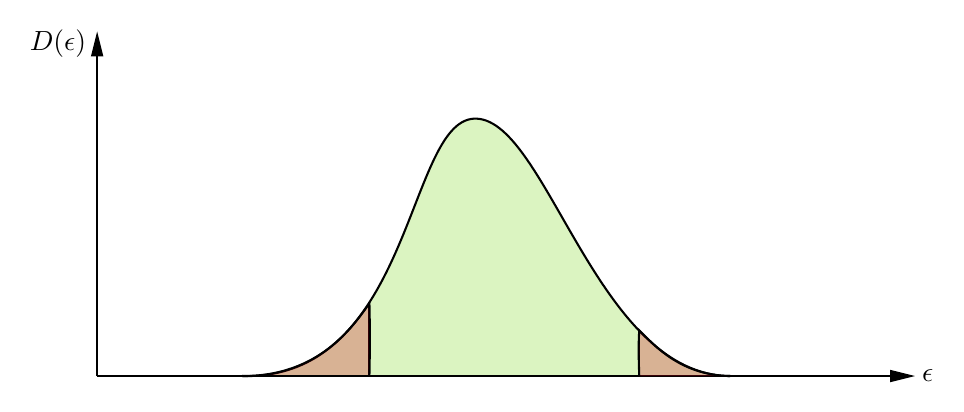
\begin{tikzpicture}[x=0.75pt,y=0.75pt,yscale=-1,xscale=1]
%uncomment if require: \path (0,300); %set diagram left start at 0, and has height of 300

%Curve Lines [id:da4027176161560928] 
\draw [fill={rgb, 255:red, 184; green, 233; blue, 134 }  ,fill opacity=0.51 ]   (155,186.17) .. controls (238,188.17) and (234,60.17) .. (268,62.17) .. controls (302,64.17) and (326.11,185.94) .. (390,186.17) ;
%Straight Lines [id:da13681751123326968] 
\draw    (85,186.17) -- (85,22.17) ;
\draw [shift={(85,20.17)}, rotate = 450] [fill={rgb, 255:red, 0; green, 0; blue, 0 }  ][line width=0.08]  [draw opacity=0] (12,-3) -- (0,0) -- (12,3) -- cycle    ;
%Straight Lines [id:da0169394948141961] 
\draw    (216.17,151.17) -- (216.17,186.17) ;
%Straight Lines [id:da6960384366783567] 
\draw    (346.17,164.17) -- (346.17,186.17) ;
%Curve Lines [id:da9091055633021599] 
\draw [fill={rgb, 255:red, 208; green, 2; blue, 27 }  ,fill opacity=0.27 ]   (155,186.17) .. controls (192,186.33) and (208.13,162.31) .. (216.17,151.17) .. controls (216.5,168.33) and (216.5,167.33) .. (216.17,186.17) ;
%Straight Lines [id:da6561575439712553] 
\draw    (85,186.17) -- (477,186.17) ;
\draw [shift={(479,186.17)}, rotate = 180] [fill={rgb, 255:red, 0; green, 0; blue, 0 }  ][line width=0.08]  [draw opacity=0] (12,-3) -- (0,0) -- (12,3) -- cycle    ;
%Curve Lines [id:da14298622888330836] 
\draw [fill={rgb, 255:red, 208; green, 2; blue, 27 }  ,fill opacity=0.27 ]   (346.17,186.17) .. controls (345.8,175.43) and (345.8,170.23) .. (346.17,164.17) .. controls (352.2,169.83) and (365,185.83) .. (390,186.17) ;

% Text Node
\draw (481,186.17) node [anchor=west] [inner sep=0.75pt]    {$\epsilon $};
% Text Node
\draw (81.21,26) node [anchor=east] [inner sep=0.75pt]    {$D( \epsilon )$};


\end{tikzpicture}